% Add the listed directories to the search path
% (allows easy moving around later)
% warning: these paths are searched AFTER local config kpsewhich
\makeatletter
\def\input@path{{./.resources/latex/}{./.resources/texmf-local/tex/latex}{./resources/texmf-local/tex/bibtex}{./.resources/econ-ark}{./Resources/LaTeXInputs/}{./Resources/texmf-local/tex/latex/}}
\makeatother 
\documentclass[SolvingMicroDSOPs]{subfiles}
% econtexRoot gets obliterated by the documentclass command 
%\input{./.econtexRoot}\documentclass[SolvingMicroDSOPs]{subfiles}
\input{./.econtexRoot}\onlyinsubfile{% https://tex.stackexchange.com/questions/463699/proper-reference-numbers-with-subfiles
    \csname @ifpackageloaded\endcsname{xr-hyper}{%
      \externaldocument{\econtexRoot/SolvingMicroDSOPs}% xr-hyper in use; optional argument for url of main.pdf for hyperlinks
    }{%
      \externaldocument{\econtexRoot/SolvingMicroDSOPs}% xr in use
    }%
    \renewcommand\labelprefix{}%
    % Initialize the counters via the labels belonging to the main document:
}



% Get xrefs; only works properly if main file has already been successfully compiled
\onlyinsubfile{\externaldocument{SolvingMicroDSOPs}} 



\begin{document}

\hypertarget{solving-the-next-to-last-period}{}
\hypertarget{solving-the-next}{}
\section{Solving the Next-to-Last Period}\label{sec:solving-the-next}

To reduce clutter, we now temporarily assume that $\PermGroFac_{\prd}=1$ for all $\prd$, so that the $\PermGroFac$ terms from the earlier derivations disappear, and setting $t=T$ the problem in the second-to-last period of life can now be expressed as
\begin{verbatimwrite}{./Equations/vEndTm1.tex}
\begin{equation}\begin{gathered}\begin{aligned}
  \vFunc_{\MidPrdLsT}(\mNrm)  & = \max_{\cNrm} ~~ \uFunc(\cNrm) +
                              \vEndPrdLsT(\overbrace{\mNrm-\cNrm}^{\aNrm})
                              \label{eq:vEndTm1}
\end{aligned}\end{gathered}\end{equation}
\end{verbatimwrite}
%\renewcommand{\stge}{T}
  \begin{equation}\begin{gathered}\begin{aligned}
        {\vFunc}_{\MidStepm}({m}_{\stge-1})   & = \max_{\cNrm_{\stge-1}}
        \left\{
          \frac{{c}_{\stge-1}^{1-\CRRA}}{1-\CRRA} +
          \vFunc_{\BegStepm}({m}_{\stge-1}-{c}_{\stge-1})
        \right\}.
        \label{eq:vEndTm1}
      \end{aligned}\end{gathered}\end{equation}%\renewcommand{\stge}{t}
\unskip
where 
\begin{equation*}\begin{gathered}\begin{aligned}
  \vFunc_{\EndPrdLsT}(\aNrm)  & = \DiscFac \vFunc_{\BegPrd}(\aNrm) 
\\                          & = \DiscFac \Ex_{\BegPrd} \left[\PermGroFacAdjV \vFunc_{\MidPrd}(\underbrace{\aNrm \RNrm_{\prdT} + \TranShkEmp_{\prdT}}_{{m}_{\prdT}})\right]
    \end{aligned}\end{gathered}\end{equation*}

% \begin{equation*}\begin{gathered}\begin{aligned}
%       \vFunc_{\prdLsT}(\mNrm)  & = \max_{\cNrm} ~~ \uFunc(\cNrm) 
%      + \DiscFac \Ex_{\EndPrdLsT} \left[\PermGroFacAdjV \vFunc_{\MidPrd}(\underbrace{(\mNrm-\cNrm)\RNrm_{\prdT} + \TranShkEmp_{\prdT}}_{{m}_{\prdT}})\right].
%     \end{aligned}\end{gathered}\end{equation*}


Using (0) $\prd=\trmT$; (1) $\vFunc_{\prdT}(m)=\uFunc(m)$; (2) the definition of $\uFunc(m)$; and (3) the definition of the expectations operator,  %\newcommand{\TranShkEmpDummy}{\vartheta}
\begin{equation}\begin{gathered}\begin{aligned}
      \vFunc_{\BegPrd}(\aNrm)   & = \PermGroFacAdjV\int_{0}^{\infty} \frac{\left(\aNrm \RNrm_{\prd}+ \TranShkEmpDummy\right)^{1-\CRRA}}{1-\CRRA}  d\FDist(\TranShkEmpDummy) \label{eq:NumDefInt}
    \end{aligned}\end{gathered}\end{equation}
where $\FDist(\TranShkEmp)$ is the cumulative distribution function for ${\TranShkEmp}$.

\lstset{basicstyle=\ttfamily\footnotesize,breaklines=true,language=Python,frame=single}
\lstinputlisting{./Code/Python/snippets/rawsolution.py}

This maximization problem implicitly defines a `local function' $\cFunc_{\prdT-1}(\mNrm)$ that yields optimal consumption in period $\prdt-1$ for any specific numerical level of resources like $m=1.7$.%  (When we need to use this function from some context outside of the local context in which it was solved, we can reference by its absolute index, $\cFunc_{\prdT-1}$).

But because there is no general analytical solution to this problem, for any given $m$ we must use numerical computational tools to find the $\cNrm$ that maximizes the expression.  This is excruciatingly slow because for every potential $c$ to be considered, a definite integral over the interval $(0,\infty)$ must be calculated numerically, and numerical integration is \textit{very} slow (especially over an unbounded domain!).

\hypertarget{discretizing-the-distribution}{}
\subsection{Discretizing the Distribution}
Our first speedup trick is therefore to construct a discrete approximation to the lognormal distribution that can be used in place of numerical integration.  That is, we want to approximate the expectation over $\TranShkEmp$ of a function $g(\TranShkEmp)$ by calculating its value at set of $n_{\TranShkEmp}$ points $\TranShkEmp_{i}$, each of which has an associated probability weight $w_{i}$:
\begin{equation*}\begin{gathered}\begin{aligned}
      \Ex[g(\TranShkEmp)] & = \int_{\TranShkEmpMin}^{\TranShkEmpMax}(\TranShkEmpDummy)d\FDist(\TranShkEmpDummy) \\
      & \approx \sum_{\TranShkEmp = 1}^{n}w_{i}g(\TranShkEmp_{i})
    \end{aligned}\end{gathered}\end{equation*}
(because adding $n$ weighted values to each other is enormously faster than general-purpose numerical integration).

Such a procedure is called a `quadrature' method of integration; \cite{Tanaka2013-bc} survey a number of options, but for our purposes we choose the one which is easiest to understand: An `equiprobable' approximation (that is, one where each of the values of $\TranShkEmp_{i}$ has an equal probability, equal to $1/n_{\TranShkEmp}$).

We calculate such an $n$-point approximation as follows.

Define a set of points from $\sharp_{0}$ to $\sharp_{n_{\TranShkEmp}}$ on the $[0,1]$ interval
as the elements of the set $\sharp = \{0,1/n,2/n, \ldots,1\}$.\footnote{These points define intervals that constitute a partition of the domain of $\FDist$.}  Call the inverse of the $\TranShkEmp$ distribution $\FDist^{-1}_{\phantom{\TranShkEmp}}$, and define the
points $\sharp^{-1}_{i} = \FDist^{-1}_{\phantom{\TranShkEmp}}(\sharp_{i})$.  Then
the conditional mean of $\TranShkEmp$ in each of the intervals numbered 1 to $n$ is:
\begin{equation}\begin{gathered}\begin{aligned}
      \TranShkEmp_{i} \equiv \Ex[\TranShkEmp | \sharp_{i-1}^{-1} \leq \TranShkEmp < \sharp_{i}^{-1}]  & = \int_{\sharp^{-1}_{i-1}}^{\sharp^{-1}_{i}} \vartheta ~ d\FDist_{\phantom{\TranShkEmp}}(\vartheta)  ,
    \end{aligned}\end{gathered}\end{equation}
and when the integral is evaluated numerically for each $i$ the result is a set of values of $\TranShkEmp$ that correspond to the mean value in each of the $n$ intervals.

The method is illustrated in Figure~\ref{fig:discreteapprox}.  The solid continuous curve represents
the ``true'' CDF $\FDist(\TranShkEmp)$ for a lognormal distribution such that $\Ex[\TranShkEmp] = 1$, $\sigma_{\TranShkEmp} = 0.1$.  The short vertical line segments represent the $n_{\TranShkEmp}$
equiprobable values of $\TranShkEmp_{i}$ which are used to approximate this
distribution.\footnote{More sophisticated approximation methods exist
  (e.g.\ Gauss-Hermite quadrature; see \cite{kopecky2010finite} for a discussion of other alternatives), but the method described here is easy to understand, quick to calculate, and has additional advantages briefly described in the discussion of simulation below.}
\begin{verbatimwrite}{./Figures/discreteApprox.tex}
  \hypertarget{discreteApprox}{}
  \begin{figure}
    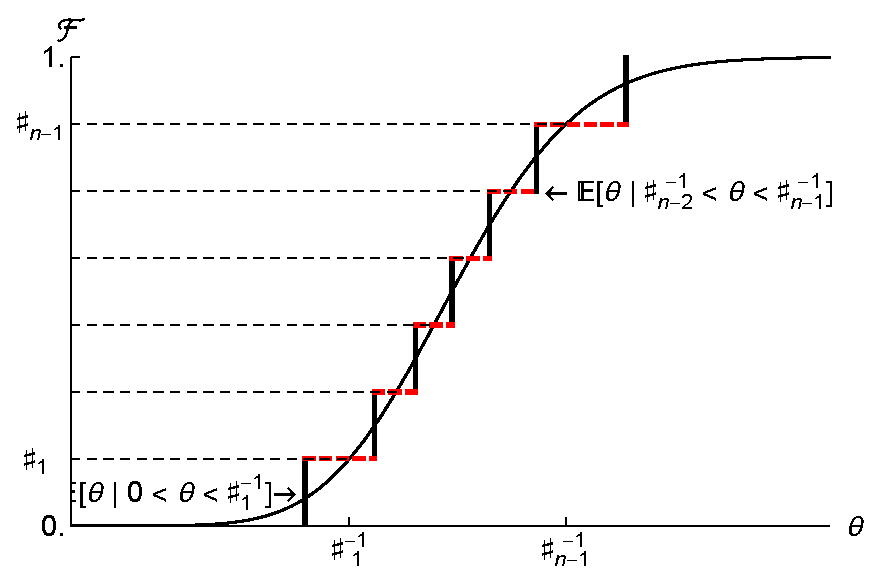
\includegraphics[width=0.8\textwidth]{./Figures/discreteApprox}
    \caption{Equiprobable Discrete Approximation to Lognormal Distribution $\FDist$}
    \label{fig:discreteapprox}
  \end{figure}
\end{verbatimwrite}
  \hypertarget{discreteApprox}{}
  \begin{figure}
    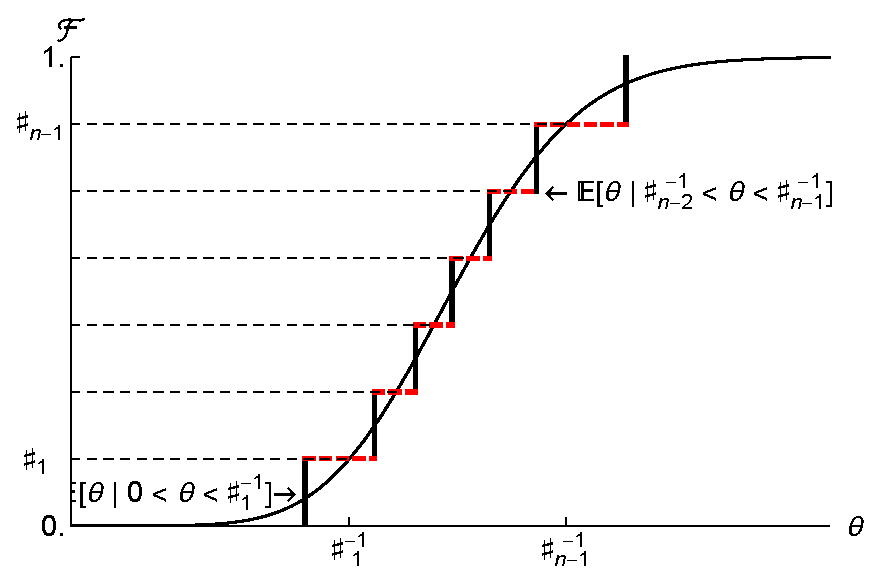
\includegraphics[width=6in]{./Figures/discreteApprox}
    \caption{Equiprobable Discrete Approximation to Lognormal Distribution $\FDist$}
    \label{fig:discreteapprox}
  \end{figure}
\unskip



Because one of the purposes of these notes is to connect the math to the code that solves the math, we display here a brief snippet from the notebook that constructs these points.


\lstset{basicstyle=\ttfamily\footnotesize,breaklines=true,language=Python,frame=single}
\lstinputlisting{./Code/Python/snippets/equiprobable-make.py}\nopagebreak

\begin{verbatimwrite}{./Equations/vDiscrete.tex}
  \begin{equation}\begin{gathered}\begin{aligned}
        \vFunc_{{\prdLst}_\cntn}(\aNrm)  & =   \DiscFac \PermGroFacAdjV\left(\frac{1}{n_{\TranShkEmp}}\right)\sum_{i=1}^{n_{\TranShkEmp}}   \frac{\left(\RNrm_{\prd} \aNrm + \TranShkEmp_{i}\right)^{1-\CRRA}}{1-\CRRA} \label{eq:vDiscrete}
      \end{aligned}\end{gathered}\end{equation}
\end{verbatimwrite}

We now substitute our approximation \eqref{eq:vDiscrete} for $\vEndPrdLsT(a)$ in \eqref{eq:vEndTm1} which is simply the sum of $n_{\TranShkEmp}$ numbers and is therefore easy to calculate (compared to the full-fledged numerical integration \eqref{eq:NumDefInt} that it replaces).

  \begin{equation}\begin{gathered}\begin{aligned}
        \vFunc_{{\cntn}(\prdLst)}(\aNrm)  & =   \DiscFac \PermGroFacAdjV\left(\frac{1}{n_{\tranShkEmp}}\right)\sum_{i=1}^{n_{\tranShkEmp}}   \frac{\left(\RNrmByG_{\prdt} \aNrm + \tranShkEmp_{i}\right)^{1-\CRRA}}{1-\CRRA} \label{eq:vDiscrete}
\UnifiedNote{Numerical approximation of ℰ(xₑ) using discrete Pₐᵥ = {1/n,...,1/n} over 𝒵ₐᵥ = {ζ₁,...,ζₙ}}
      \end{aligned}\end{gathered}\end{equation}
\unskip
% so we can rewrite the maximization problem that defines the middle step of period {$\prdLst$} as
% \begin{verbatimwrite}{./Equations/vEndTm1.tex}
%   \begin{equation}\begin{gathered}\begin{aligned}
%         \vFunc_{\MidPrdLsT}(\mNrm)   & = \max_{\cNrm}
%         \left\{
%           \frac{\cNrm^{1-\CRRA}}{1-\CRRA} +
%           \vFunc_{\MidPrd}(\mNrm-\cNrm)
%         \right\}.
%         \label{eq:vEndTm1}
%       \end{aligned}\end{gathered}\end{equation}
% \end{verbatimwrite}
% %\renewcommand{\stge}{T}
  \begin{equation}\begin{gathered}\begin{aligned}
        {\vFunc}_{\MidStepm}({m}_{\stge-1})   & = \max_{\cNrm_{\stge-1}}
        \left\{
          \frac{{c}_{\stge-1}^{1-\CRRA}}{1-\CRRA} +
          \vFunc_{\BegStepm}({m}_{\stge-1}-{c}_{\stge-1})
        \right\}.
        \label{eq:vEndTm1}
      \end{aligned}\end{gathered}\end{equation}%\renewcommand{\stge}{t}
\unskip

\lstinputlisting{./Code/Python/snippets/equiprobable-max-using.py}

\begin{comment}
  In the {\SMDSOPntbk} notebook, the section ``Discretization of the Income Shock Distribution'' provides code that instantiates the \texttt{DiscreteApproximation} class defined in the \texttt{resources} module. This class creates a 7-point discretization of the continuous log-normal distribution of transitory shocks to income by utilizing seven points, where the mean value is $-.5 \sigma^2$, and the standard deviation is $\sigma = .5$.

  A close look at the \texttt{DiscreteApproximation} class and its subclasses should convince you that the code is simply a computational implementation of the mathematical description of equiprobable discrete approximation in this section. Moreover, the Python code generates a graph of the discretized distribution depicted in \ref{fig:discreteapprox}.
\end{comment}

\hypertarget{the-approximate-consumption-and-value-functions}{}
\subsection{The Approximate Consumption and Value Functions}

Given any particular value of $\mNrm$, a numerical maximization tool can now find the $\cNrm$ that solves \eqref{eq:vEndTm1} in a reasonable amount of time.

\begin{comment}
  % The {\SMDSOPntbk} notebook follows a series of steps to achieve this. Initially, parameter values for the coefficient of relative risk aversion (CRRA, $\rho$), the discount factor ($\beta$), the permanent income growth factor ($\PermGroFac$), and the risk-free interest rate ($R$ are specified in ``Define Parameters, Grids, and the  Utility Function.'')

  % After defining the utility function, the `natural borrowing constraint' is defined as $\underline{a}_{\prdT-1}=-\underline{\TranShkEmp}\RNrm_{\prdT}^{-1}$, which will be discussed in greater depth in section \ref{subsec:LiqConstrSelfImposed}. %Following the reformulation of the maximization problem, an instance of the \texttt{gothic\_class} is created using the specifications and the discretized distribution described in the prior lines of code; this is required to provide the numerical solution.
\end{comment}

The notebook code responsible for computing an estimated consumption function begins in ``Solving the Model by Value Function Maximization,'' where a vector containing a set of possible values of market resources $m$ is created (in the code, various $m$ vectors have names beginning {\mVec}; in these notes we will use boldface italics to represent vectors, so we can refer to our collection of $m$ points as $\vctr{m}$ with values indexed by brackets: $\vctr{m}[1]$ is the first entry in the vector, up to a last entry $\vctr{m}[-1]$; we arbitrarily (and suboptimally) pick the first five integers as our five {\mVec}  gridpoints (in the code, \code{mVec\_int}= $\{0.,1.,2.,3.,4.\}$)).

% Finally, the previously computed values of optimal $c$ and the grid of market resources are combined to generate a graph of the approximated consumption function for this specific instance of the problem. To reduce the computational challenge of solving the problem, the process is evaluated only at a small number of gridpoints.


\hypertarget{an-interpolated-consumption-function}{}
\subsection{An Interpolated Consumption Function} \label{subsec:LinInterp}


This is accomplished in ``An Interpolated Consumption Function,'' which generates an interpolating function that we designate $\Aprx{\cFunc}_{\MidPrdLsT}(\mNrm)$. %When called with an $\mNrm$ that is equal to one of the points in $\code{{{\mVec}\_int}}$, $\Aprx{\cFunc}_{\prdT-1}$ returns the associated value of $\vctr{c}_{\code{\prdT-1}}$, and when called with a value of $\mNrm$ that is not exactly equal to one of the \texttt{mVec\_int}, returns the value of $c$ that reflects a linear interpolation between the $\vctr{c}_{\code{\prdT-1}}$ points associated with the two \texttt{mVec\_int} points immediately above and below $\mNrm$.  


Figures \ref{fig:PlotcTm1Simple} and~\ref{fig:PlotVTm1Simple} show
plots of the constructed $\Aprx{\cFunc}_{\prdT-1}$ and $\Aprx{\vFunc}_{\prdT-1}$. While the $\Aprx{\cFunc}_{\prdT-1}$ function looks very smooth, the fact that the $\Aprx{\vFunc}_{\prdT-1}$ function is a set of line segments is very evident.  This figure provides the beginning of the intuition for why trying to approximate the value function directly is a bad idea (in this context).\footnote{For some problems, especially ones with discrete choices, value function approximation is unavoidable; nevertheless, even in such problems, the techniques sketched below can be very useful across much of the range over which the problem is defined.}

\hypertarget{PlotcTm1Simple}{}
\begin{figure}
  \centerline{\includegraphics[width=6in]{./Figures/PlotcTm1Simple}}
  \caption{$\cFunc_{\trmT-1}(\mNrm)$ (solid) versus $\Aprx{\cFunc}_{\trmT-1}(\mNrm)$ (dashed)}
  \label{fig:PlotcTm1Simple}
\end{figure}

\hypertarget{PlotvTm1Simple}{}
\begin{figure}
  \centerline{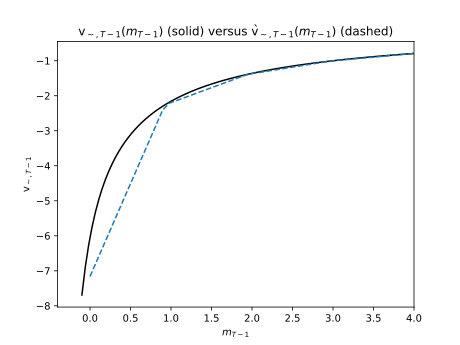
\includegraphics[width=6in]{./Figures/PlotVTm1Simple}}
  \caption{$\vFunc_{\trmT-1}$ (solid) versus $\Aprx{\vFunc}_{\trmT-1}(\mNrm)$ (dashed)}
  \label{fig:PlotVTm1Simple}
\end{figure}



\hypertarget{interpolating-expectations}{}
\subsection{Interpolating Expectations}


Piecewise linear `spline' interpolation as described above works well for generating a good approximation to the true optimal consumption function. However, there is a clear inefficiency in the program: Since it uses equation \eqref{eq:vEndTm1}, for every value of $\mNrm$ the program must calculate the utility consequences of various possible choices of $\cNrm$ (and therefore $\aNrm_{\prdT-1}$) as it searches for the best choice.

For any given index $j$ in $\vctr{m}[j]$, the algorithm, as it searches for the corresponding optimal $a$, the algorithm will end up  calculating $\vFunc_{\EndPrdLsT}(\tilde{a})$ for many $\tilde{a}$ values close to the optimal $a_{\prdT-1}$.  Indeed, even when searching for the optimal $a$ for a \emph{different} $m$ (say $\vctr{m}[k]$ for $k \neq j$) the search process might compute $\vFunc_{\EndPrdLsT}(a)$ for an $a$ close to the correct optimal $a$ for $\vctr{m}[j]$. But if that difficult computation does not correspond to the exact solution to the $\vctr{m}[k]$ problem, it is discarded.  

% (These lists contain the points of the $\vctr{a}_{\prdT-1}$ and $\vctr{v}_{\prdT-1}$ vectors, respectively.)

The notebook section ``Interpolating Expectations,'' now interpolates the expected value of \textit{ending} the period with a given amount of assets.\footnote{What we are doing here is closely related to `the method of parameterized expectations' of \cite{denHaanMarcet:parameterized}; the only difference is that our method is essentially a nonparametric version.}  %The problem is solved in the same block with the remaining lines of code.

Figure~\ref{fig:PlotOTm1RawVSInt} compares the true value function to the approximation produced by following the interpolation procedure; the approximated and exact functions are of course identical at the gridpoints of $\vctr{a}$ and they appear reasonably close except in the region below $\mNrm=1$.

\hypertarget{PlotOTm1RawVSInt}{}
\begin{figure}
  \centerline{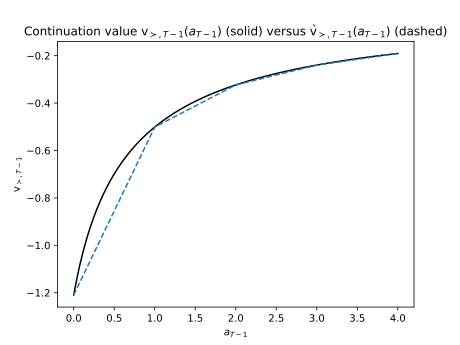
\includegraphics[width=6in]{./Figures/PlotOTm1RawVSInt}}
  \caption{End-Of-Period Value $\vFunc_{(\prdT-1)_\cntn}(a_{\prdT-1})$ (solid) versus $\Aprx{\vFunc}_{({\trmT-1})_\cntn}(a_{\trmT-1})$ (dashed)}
  \label{fig:PlotOTm1RawVSInt}
\end{figure}

\hypertarget{PlotComparecTm1AB}{}
\begin{figure}
  \centerline{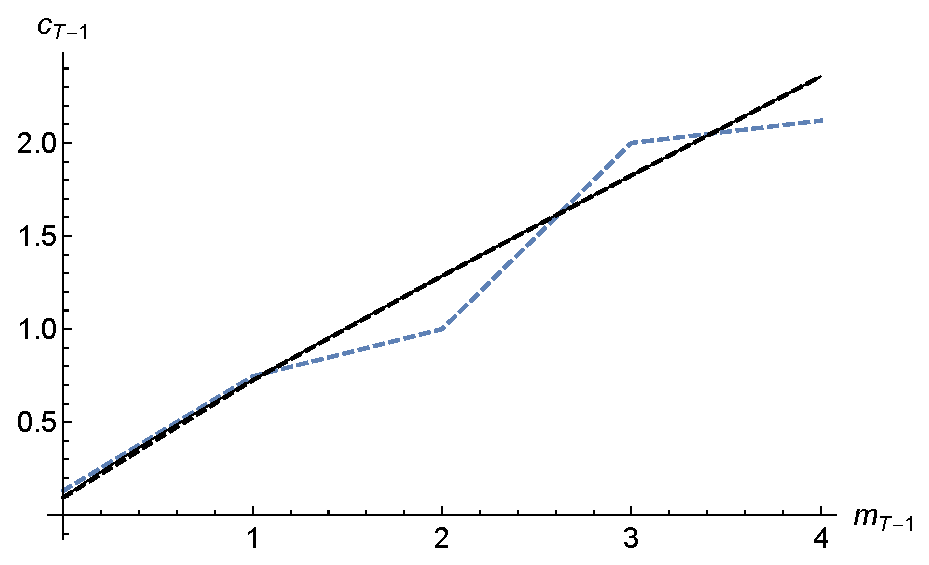
\includegraphics[width=6in]{./Figures/PlotComparecTm1AB}}
  \caption{$\cFunc_{\trmT-1}(\mNrm)$ (solid) versus $\Aprx{\cFunc}_{\trmT-1}(\mNrm)$ (dashed)}
  \label{fig:PlotComparecTm1AB}
\end{figure}

\Fix{\marginpar{\tiny In all figs, replace gothic h with notation corresponding to the lecture notes.}}

Nevertheless, the consumption rule obtained when the approximating $\Aprx{\vFunc}_{(\prdT-1)_\cntn}(a_{\prdT-1})$ is used instead of $\vFunc_{(\prdT-1)_\cntn}(a_{\prdT-1})$ is surprisingly bad, as shown in figure \ref{fig:PlotComparecTm1AB}.  For example, when $\mNrm$ goes from 2 to 3, $\Aprx{\cFunc}_{\prdT-1}$ goes from about 1 to about 2, yet when $\mNrm$ goes from 3 to 4, $\Aprx\cNrm$ goes from about 2 to about 2.05.  The function fails even to be concave, which is distressing because Carroll and Kimball~\citeyearpar{ckConcavity} prove that the correct consumption function is strictly concave in a wide class of problems that includes this one.

\hypertarget{value-function-versus-first-order-condition}{}
\subsection{Value Function versus First Order Condition}\label{subsec:vVsuP}

Loosely speaking, our difficulty reflects the fact that the
consumption choice is governed by the \textit{marginal} value function,
not by the \textit{level} of the value function (which is the object that
we approximated).  To understand this point, recall that a quadratic
utility function
exhibits risk aversion because with a stochastic $c$,
\begin{equation}
  \Ex[-(c - \cancel{c})^{2}] < - (\Ex[c] - \cancel{c})^{2}
\end{equation}
(where $\cancel{c}$ is the `bliss point' which is assumed always to exceed feasible $c$). However, unlike the CRRA utility function,
with quadratic utility the consumption/saving \textit{behavior} of consumers
is unaffected by risk since behavior is determined by the first order condition, which
depends on \textit{marginal} utility, and when utility is quadratic, marginal utility is unaffected
by risk:
\begin{equation}
  \Ex[-2(c - \cancel{c})] = - 2(\Ex[c] - \cancel{c}).
\end{equation}

Intuitively, if one's goal is to accurately capture choices
that are governed by marginal value,
numerical techniques that approximate the \textit{marginal} value
function will yield a more accurate approximation to
optimal behavior than techniques that approximate the \textit{level}
of the value function.

The first order condition of the maximization problem in period $\trmT-1$ is:
\begin{verbatimwrite}{./Equations/FOCTm1.tex}
  \begin{equation}\begin{gathered}\begin{aligned}
        \uFunc^{c}(\cNrm)       & = \DiscFac \Ex_{\cntn(T-1)} [\PermGroFacAdjMu\Rfree \uFunc^{c}(c_{\prdT})]  %\label{eq:focraw}
        \\      \cNrm^{-\CRRA}   & = \Rfree \DiscFac \left(\frac{1}{n_{\TranShkEmp}}\right) \sum_{i=1}^{n_{\TranShkEmp}} \PermGroFacAdjMu\left(\Rfree (\mNrm-\cNrm) + \TranShkEmp_{i}\right)^{-\CRRA} \label{eq:FOCTm1}.
      \end{aligned}\end{gathered}\end{equation}
\end{verbatimwrite}
  \begin{equation}\begin{gathered}\begin{aligned}
        \uFunc^{{c}}(\cNrm)       & = \DiscFac \Ex_{\cntn(T-1)} [\PermGroFacAdjMu\Rfree \uFunc^{{c}}({c}_{\prdT})]  %\label{eq:focraw}
        \\      \cNrm^{-\CRRA}   & = \Rfree \DiscFac \left(\frac{1}{n_{\TranShkEmp}}\right) \sum_{i=1}^{n_{\TranShkEmp}} \PermGroFacAdjMu\left(\Rfree (\mNrm-\cNrm) + \TranShkEmp_{i}\right)^{-\CRRA} \label{eq:FOCTm1}.
      \end{aligned}\end{gathered}\end{equation}
\unskip
\hypertarget{PlotuPrimeVSOPrime}{}
\begin{figure}
  \centerline{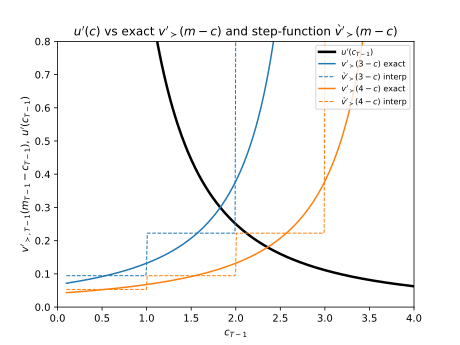
\includegraphics[width=6in]{./Figures/PlotuPrimeVSOPrime}}
  \caption{$\uFunc^{c}(c)$ versus $\vFunc_{({\trmT-1})_\cntn}^{a}(3-c), \vFunc_{({\trmT-1})_\cntn}^{a}(4-c), \Aprx{\vFunc}_{({\trmT-1})_\cntn}^{a}(3-c), \Aprx{\vFunc}_{({\trmT-1})_\cntn}^{a}(4-c)$}
  \label{fig:PlotuPrimeVSOPrime}
\end{figure}



The downward-sloping curve in Figure \ref{fig:PlotuPrimeVSOPrime}
shows the value of $\cNrm^{-\CRRA}$ for our baseline parameter values
for $0 \leq \cNrm \leq 4$ (the horizontal axis).  The solid
upward-sloping curve shows the value of the RHS of (\ref{eq:FOCTm1})
as a function of $\cNrm$ under the assumption that $\mNrm=3$.
Constructing this figure is time-consuming, because for every
value of $\cNrm$ plotted we must calculate the RHS of
(\ref{eq:FOCTm1}).  The value of $\cNrm$ for which the RHS and LHS
of (\ref{eq:FOCTm1}) are equal is the optimal level of consumption
given that $\mNrm=3$, so the intersection of the downward-sloping
and the upward-sloping curves gives the (approximated) optimal value of $\cNrm$.
As we can see, the two curves intersect just below $\cNrm=2$.
Similarly, the upward-sloping dashed curve shows the expected value
of the RHS of (\ref{eq:FOCTm1}) under the assumption that $\mNrm=4$,
and the intersection of this curve with $\uFunc^{c}(\cNrm)$ yields the
optimal level of consumption if $\mNrm=4$.  These two curves
intersect slightly below $\cNrm=2.5$.  Thus, increasing $\mNrm$
from 3 to 4 increases optimal consumption by about 0.5.

Now consider the derivative of our function $\Aprx{\vFunc}_{(\prdT-1)}(a_{\prdT-1})$.  Because we have
constructed $\Aprx{\vFunc}_{(\prdT-1)}$ as a linear interpolation, the slope of
$\Aprx{\vFunc}_{(\prdT-1)}(a_{\prdT-1})$ between any two adjacent points
$\{\vctr{a}[i],\vctr{},\vctr{a}[{i+1}]\}$ is constant.  The level of the slope immediately below any
particular gridpoint is different, of course, from the slope above that gridpoint, a fact which
implies that the derivative of $\Aprx{\vFunc}_{(\prdT-1)_\cntn}(a_{\prdT-1})$ follows a step function.

The solid-line step function in Figure \ref{fig:PlotuPrimeVSOPrime} depicts the actual value of
$\Aprx{\vFunc}_{(\prdT-1)_\cntn}^{a}(3-\cNrm)$.  When we attempt to find optimal values of
$\cNrm$ given $\mNrm$ using $\Aprx{\vFunc}_{(\prdT-1)_\cntn}(a_{\prdT-1})$, the numerical optimization routine will
return the $\cNrm$ for which
$\uFunc^{c}(\cNrm) = \Aprx{\vFunc}^{a}_{(\prdT-1)_\cntn}(\mNrm-\cNrm)$.  Thus, for
$\mNrm=3$ the program will return the value of $\cNrm$ for which the downward-sloping
$\uFunc^{c}(\cNrm)$ curve intersects with the
$\Aprx{\vFunc}_{(\prdT-1)_\cntn}^{a}(3-\cNrm)$; as the diagram shows, this value is exactly equal to 2.
Similarly, if we ask the routine to find the optimal $\cNrm$ for $\mNrm=4$, it finds the point of
intersection of $\uFunc^{c}(\cNrm)$ with $\Aprx{\vFunc}_{(\prdT-1)_\cntn}^{a}(4-\cNrm)$; and as the diagram shows, this
intersection is only slightly above 2.  Hence, this figure illustrates why the numerical consumption
function plotted earlier returned values very close to $\cNrm=2$ for both $\mNrm=3$ and $\mNrm=4$.

We would obviously obtain much better estimates of the point of intersection between $\uFunc^{c}(\cNrm)$ and $\vFunc_{(\prdT-1)_\cntn}^{a}(\mNrm-\cNrm)$ if our estimate of $\Aprx{\vFunc}^{a}_{(\prdT-1)_\cntn}$ were not a step function.  In fact, we already know how to construct linear interpolations to functions, so the obvious next step is to construct a linear interpolating approximation to the \textit{expected marginal value of end-of-period assets function} at the points in $\vctr{a}$:
\begin{equation}\begin{gathered}\begin{aligned}
      \vFunc_{(\prdT-1)_\cntn}^{a}(\vctr{a})  & =  \DiscFac \Rfree \PermGroFacAdjMu \left(\frac{1}{n_{\TranShkEmp}}\right) \sum_{i=1}^{n_{\TranShkEmp}} \left(\RNrm_{\prdT} \vctr{a} + \TranShkEmp_{i}\right)^{-\CRRA} \label{eq:vEndPrimeTm1}
    \end{aligned}\end{gathered}\end{equation}
yielding $\vctr{v}{^{a}_{(\prdT-1)_\cntn}}$ (the vector of expected end-of-period-$(T-1)$ marginal values of assets corresponding to \code{aVec}),  %$\{\{\vctr{a}}\code{_{\prdT-1}},\vFunc_{(\prdT-1)_\cntn}^{a}(\vctr{{a}[1]}_{\prdT-1}\},\{\vctr{a}_{(T-1)},\vFunc_{(\prdT-1)_\cntn}^{a}\}\ldots\}$
and construct
$\Aprx{\vFunc}_{(\prdT-1)_\cntn}^{a}(a_{\prdT-1})$ as the linear
interpolating function that fits this set of points.

\hypertarget{PlotOPRawVSFOC}{}
\begin{figure}
  \centerline{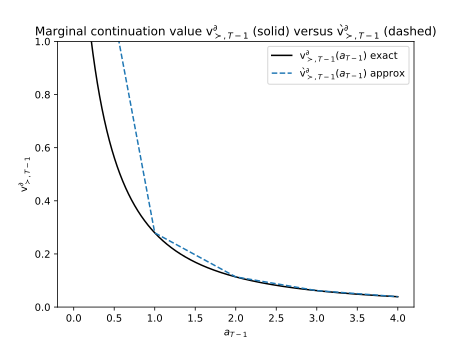
\includegraphics[width=6in]{./Figures/PlotOPRawVSFOC}}
  \caption{$\vFunc_{(\prdT-1)_\cntn}^{a}(a_{\prdT-1})$ versus $\Aprx{\vFunc}_{(\prdT-1)_\cntn}^{a}(a_{\prdT-1})$}
  \label{fig:PlotOPRawVSFOC}
\end{figure}

% This is done by making a call to the \texttt{InterpolatedUnivariateSpline} function, passing it \code{aVec} and \texttt{vpVec} as arguments. Note that in defining the list of values \texttt{vpVec}, we again make use of the predefined \texttt{gothic.VP\_Tminus1} function. These steps are the embodiment of equation~(\ref{eq:vEndPrimeTm1}), and construct the interpolation of the expected marginal value of end-of-period assets as described above.

The results are shown in Figure \ref{fig:PlotOPRawVSFOC}.  The linear interpolating approximation looks roughly as good (or bad) for the \textit{marginal} value function as it was for the level of the value function. However, Figure \ref{fig:PlotcTm1ABC} shows that the new consumption function (long dashes) is a considerably better approximation of the true consumption function (solid) than was the consumption function obtained by approximating the level of the value function (short dashes).

\hypertarget{PlotcTm1ABC}{}
\begin{figure}
  \centerline{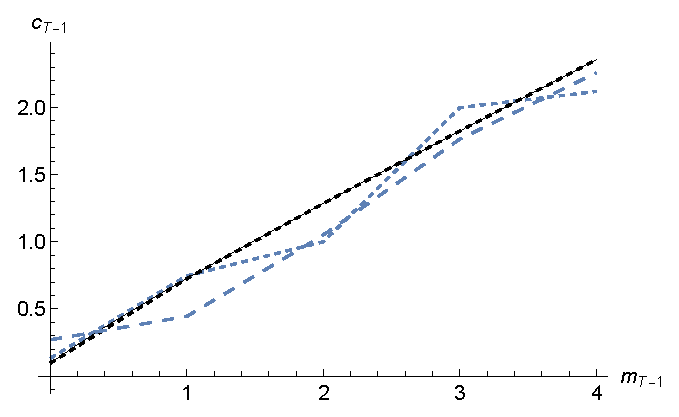
\includegraphics[width=6in]{./Figures/PlotcTm1ABC}}
  \caption{$\cFunc_{\prdT-1}(\mNrm)$ (solid) Versus Two Methods for Constructing $\Aprx{\cFunc}_{\prdT-1}(\mNrm)$}
  \label{fig:PlotcTm1ABC}
\end{figure}

\hypertarget{transformation}{}
\subsection{Transformation}\label{subsec:transformation}

Even the new-and-improved consumption function diverges notably from the true
solution, especially at lower values of $m$.  That is because the
linear interpolation does an increasingly poor job of capturing the
nonlinearity of $\vFunc_{(\prdT-1)_\cntn}^{a}(a_{\prdT-1})$ at
lower and lower levels of $a$.

This is where we unveil our next trick.  To understand the logic,
start by considering the case where $\RNrm_{\prdT} = \DiscFac =
\PermGroFac_{\prdT} = 1$ and there is no uncertainty
(that is, we know for sure that income next period
will be $\TranShkEmp_{\prdT} = 1$).  The final Euler equation (recall that we are still assuming that $\prd=\trmT$) is then:
\begin{equation}\begin{gathered}\begin{aligned}
      \cNrm_{\prdT-1}^{-\CRRA}  & = c_{\prdT}^{-\CRRA}.
    \end{aligned}\end{gathered}\end{equation}

In the case we are now considering with no uncertainty and no liquidity constraints, the optimizing consumer does not care whether a unit of income is scheduled to be received in the future period $\prdT$ or the current period $\prdT-1$; there is perfect certainty that the income will be received, so the consumer treats its PDV as equivalent to a unit of current wealth.  Total resources available at the point when the consumption decision is made is therefore are comprised of two types: current market resources $\mNrm$ and `human wealth' (the PDV of future income) of $\hNrm_{\prdT-1}=1$ (because it is the value of human wealth as of the end of the period, there is only one more period of income of 1 left).

\begin{equation}
  \vFunc^{m}_{\MidPrdLsT}(\mNrm)  = \left(\frac{\mNrm+1}{2}\right)^{-\CRRA} \label{eq:vPLin}.
\end{equation}
Of course, this is a highly nonlinear function.  However, if we raise both sides of \eqref{eq:vPLin} to the power $(-1/\CRRA)$ the result is a linear function:
\begin{equation}\begin{gathered}\begin{aligned}
      % \vInv^{m}_{\prdT-1}(\mNrm) \equiv
      \left[\vFunc^{m}_{\MidPrdLsT}(\mNrm)\right]^{-1/\CRRA}  & = \frac{\mNrm+1}{2}  .
    \end{aligned}\end{gathered}\end{equation}
This is a specific example of a general phenomenon: A theoretical literature discussed in~\cite{ckConcavity} establishes that under perfect certainty, if the period-by-period marginal utility function is of the form $\cNrm_{\prd}^{-\CRRA}$, the marginal value function will be of the form $(\gamma m_{\prd}+\zeta)^{-\CRRA}$ for some constants $\{\gamma,\zeta\}$.  This means that if we were solving the perfect foresight problem numerically, we could always calculate a numerically exact (because linear) interpolation.

To put the key insight in intuitive terms, the nonlinearity we are facing springs in large part from the fact that the marginal value function is highly nonlinear.  But we have a compelling solution to that problem, because the nonlinearity springs largely from the fact that we are raising something to the power $-\CRRA$.  In effect, we can `unwind' all of the nonlinearity owing to that operation and the remaining nonlinearity will not be nearly so great.  Specifically, applying the foregoing insights to the end-of-period value function $\vFunc^{a}_{\MidPrdLsT}(\aNrm)$, we can define an `inverse marginal value' function
\begin{equation}\begin{gathered}\begin{aligned}
      \vInv_{\prd_\cntn}^{a}(a)  & \equiv  \left(\vFunc^{a}_{\prd_\cntn}(a)\right)^{-1/\CRRA} \label{eq:cGoth}
    \end{aligned}\end{gathered}\end{equation}
which would be linear in the perfect foresight case.\footnote{There is a corresponding inverse for the value function: $\vInv_{\prd_\cntn}(a_{\prd})=((1-\CRRA)\vFunc_{\prd_\cntn})^{1/(1-\CRRA)}$, and for the marginal marginal value function etc.}  We then construct a piecewise-linear interpolating approximation to the $\vInv_{\prd}^{a}$ function, $\Aprx{\vInv}_{\prd_\cntn}^{a}(a_{\prd})$, and for any $a$ that falls in the range $\{\vctr{a}[1],\vctr{a}[-1]\}$ we obtain our approximation of marginal value from:
\begin{equation}\begin{gathered}\begin{aligned}
      \Aprx{\vFunc}_{\prd}^{a}(a) & =
      [\Aprx{\vInv}_{\prd}^{a}(a)]^{-\CRRA}
    \end{aligned}\end{gathered}\end{equation}

The most interesting thing about all of this, though, is that the $\vInv^{a}_{\prd}$ function has another interpretation. Recall our point in \eqref{eq:upEqbetaOp} that $\uFunc^{c}(c_{\prd}) = \vEndStg^{a}(m_{\prd}-c_{\prd})$.  Since with CRRA utility $\uFunc^{c}(c)=c^{-\CRRA}$, this can be rewritten
and inverted
\begin{equation}\begin{gathered}\begin{aligned}
      (c_{\prd})^{-\CRRA} & = \vEndStg^{a}(a_{\prd})
      \\ c_{\prd} & =      \left(\vEndPrd^{a}(a)\right)^{-1/\CRRA}.
    \end{aligned}\end{gathered}\end{equation}

What this means is that for any given $a$, if we can calculate the marginal value associated with ending the period with that $a$, then we can learn the level of $c$ that the consumer must have chosen if they ended up with that $a$ as the result of an optimal unconstrained choice.  This leads us to an alternative interpretation of $\vInv^{a}$. It is the function that reveals, for any ending $a$, how much the agent must have consumed to (optimally) get to that $a$.  We will therefore henceforth refer to it as the `consumed function:'
\begin{equation}\begin{gathered}\begin{aligned}
      \Aprx{\cFunc}_{\prd_\cntn}(a_{\prd}) & \equiv \Aprx{\vInv}^{a}_{\prd_\cntn}(a_{\prd}) \label{eq:consumedfn}.    
    \end{aligned}\end{gathered}\end{equation}

%\renewcommand{\prd}{T}
Thus, for example, for period $\prdLsT$ our procedure is to calculate the vector of $\vctr{c}$ points on the consumed function:
\begin{equation}\begin{gathered}\begin{aligned}
      \vctr{c} & = \cFunc_{(\prdLsT)_\cntn}(\vctr{a}) \label{eq:consumedfnvecs}     
    \end{aligned}\end{gathered}\end{equation}
with the idea that we will construct an approximation of the consumed function $\Aprx{\cFunc}_{(\prdLsT)_\cntn}(\aNrm)$ as the interpolating function connecting these $\{\vctr{a},\vctr{c}\}$ points.

\hypertarget{the-natural-borrowing-constraint-and-the-a-lower-bound}{}
\subsection{The Natural Borrowing Constraint and the $a_{\prdLsT}$ Lower Bound} \label{subsec:LiqConstrSelfImposed}

%\renewcommand{\prd}{T} 
This is the appropriate moment to ask an awkward question: How should an interpolated, approximated `consumed' function like $\Aprx{\cFunc}_{(\prdLsT)_\cntn}(a_{\prdLsT})$ be extrapolated to return an estimated `consumed' amount when evaluated at an $a_{\prdLsT}$ outside the range spanned by $\{\vctr{a}[1],...,\vctr{a}[n]\}$?


For most canned piecewise-linear interpolation tools like \href{https://docs.scipy.org/doc/scipy/tutorial/interpolate.html}{scipy.interpolate}, when the `interpolating' function is evaluated at a point outside the provided range, the algorithm extrapolates under the assumption that the slope of the function remains constant beyond its measured boundaries (that is, the slope is assumed to be equal to the slope of nearest piecewise segment \emph{within} the interpolated range); for example, if the bottommost gridpoint is $\aVecMin = \vctratm[1]$ and the corresponding consumed level is $\cMin = \cFunc_{(\prdLsT)_\cntn}(a_1)$ we could calculate the `marginal propensity to have consumed' $\varkappa_{1}=
\Aprx{\cFunc}_{(\prdLsT)_\cntn}^{a}(\aVecMin)$ and construct the approximation as the linear extrapolation below $\vctratm[1]$ from:
\begin{equation}\begin{gathered}\begin{aligned}
      \Aprx{\cFunc}_{(\prdLsT)_\cntn}(a)  &  \equiv \cMin + (a-\aVecMin)\varkappa_{1}  \label{eq:ExtrapLin}.
    \end{aligned}\end{gathered}\end{equation}

To see that this will lead us into difficulties, consider what happens to the true (not approximated) $\vFunc^{a}_{(\prdLsT)_\cntn}(a_{\prdLsT})$ as $a_{\prdLsT}$ approaches a quantity we will call the `natural borrowing constraint': $\NatBoroCnstra_{\prdLsT}=-\underline{\TranShkEmp}\RNrm_{\prdT}^{-1}$.  From
\eqref{eq:vEndPrimeTm1} we have
\begin{equation}\begin{gathered}\begin{aligned}
      \lim_{\aNrm \downarrow \NatBoroCnstra_{\prdLsT}} \vFunc^{a}_{(\prdLsT)_\cntn}(\aNrm)
      & =                                                                                         \lim_{\aNrm \downarrow \NatBoroCnstra_{\prdLsT}} \DiscFac \Rfree \PermGroFacAdjMu \left(\frac{1}{n_{\TranShkEmp}}\right) \sum_{i=1}^{n_{\TranShkEmp}} \left( \aNrm \RNrm_{\prd}+ \TranShkEmp_{i}\right)^{-\CRRA}.
    \end{aligned}\end{gathered}\end{equation}

But since $\TranShkEmpMin=\TranShkEmp_{1}$, exactly at $\aNrm=\NatBoroCnstra_{\prdLsT}$ the first term in the summation would be $(-\TranShkEmpMin+\TranShkEmp_{1})^{-\CRRA}=1/0^{\CRRA}$ which is infinity.  The reason is simple: $-\NatBoroCnstra_{\prdLsT}$ is the PDV, as of $\prdLsT$, of the \emph{minimum possible realization of income} in $\prdT$ ($\RNrm_{\prdT}\NatBoroCnstra_{\prdLsT} = -\TranShkEmp_{1}$).  Thus, if the consumer borrows an amount greater than or equal to $\underline{\TranShkEmp}\RNrm_{\prdT}^{-1}$ (that is, if the consumer ends $\prdLsT$ with $a_{\prdLsT} \leq -\underline{\TranShkEmp}\RNrm_{\prdT}^{-1}$) and then draws the worst possible income shock in period $\prdT$, they will have to consume zero in period $\prdT$, which yields $-\infty$ utility and $+\infty$ marginal utility.

As \cite{zeldesStochastic} first noticed, this means that the consumer faces a `self-imposed' (or, as above, `natural') borrowing constraint (which springs from the precautionary motive): They will never borrow an amount greater than or equal to $\underline{\TranShkEmp}\RNrm_{\prdT}^{-1}$ (that is, assets will never reach the lower bound of $\NatBoroCnstra_{\prdLsT}$).  The constraint is `self-imposed' in the precise sense that if the utility function were different (say, Constant Absolute Risk Aversion), the consumer might be willing to borrow more than $\underline{\TranShkEmp}\RNrm_{\prdT}^{-1}$ because a choice of zero or negative consumption in period $\prdT$ would yield some finite amount of utility.\footnote{Though it is very unclear what a proper economic interpretation of negative consumption might be -- this is an important reason why CARA utility, like quadratic utility, is increasingly not used for serious quantitative work, though it is still useful for teaching purposes.}

%\providecommand{\aMin}{\underline{\aNrm}}
This self-imposed constraint cannot be captured well when the $\vFunc^{a}_{(\prdLsT)_\cntn}$ function is approximated by a piecewise linear function like $\Aprx{\vFunc}^{m}_{(\prdLsT)_\cntn}$, because it is impossible for the linear extrapolation below $\aMin$ to correctly predict $\vFunc^{a}_{(\prdLsT)_\cntn}(\NatBoroCnstra_{\prdLsT})=\infty.$ %To see what will happen instead, note first that if we are approximating $\vFunc^{a}_{(\prdLsT)_\cntn}$ the smallest value in \code{aVec} must be greater than $\NatBoroCnstra_{\prdLsT}$ (because the expectation for any $a_{\prdLsT} \leq \NatBoroCnstra_{\prdLsT}$ is undefined).

% When the approximating $\vFunc^{a}_{(\prdLsT)_\cntn}$ function is evaluated at some value less than the first element in \code{aVec}, a piecewise linear approximating function will linearly extrapolate the slope that characterized the lowest segment of the piecewise linear approximation (between \texttt{aVec[1]} and \texttt{aVec[2]}), a procedure that will return a positive finite number, even if the requested $a_{\prdLsT}$ point is below $\NatBoroCnstra_{\prdLsT}$.  This means that the precautionary saving motive is understated, and by an arbitrarily large amount as the level of assets approaches its true theoretical minimum $\NatBoroCnstra_{\prdLsT}$.

%\renewcommand{\prd}{T}
So, the marginal value of saving approaches infinity as $\aNrm \downarrow \NatBoroCnstra_{\prdLsT}=-\underline{\TranShkEmp}\RNrm_{\prdT}^{-1}$.  But this implies that $\lim_{\aNrm \downarrow \NatBoroCnstra_{\prdLsT}} \cFunc_{(\prdLsT)_\cntn}(\aNrm) = (\vFunc^{a}_{(\prdLsT)_\cntn}(\aNrm))^{-1/\CRRA} = 0$; that is, as $a$ approaches its `natural borrowing constraint' minimum possible value, the corresponding amount of worst-case $c$ must approach \textit{its} lower bound: zero.

The upshot is a realization that all we need to do to address these problems is to prepend each of the $\vctr{a}_{\code{\prdLsT}}$ and $\vctr{c}_{\code{\prdLsT}}$ from \eqref{eq:consumedfnvecs} with an extra point so that the first element in the mapping that produces our interpolation function is $\{\NatBoroCnstra_{\prdLsT},0.\}$. This is done in section ``The Self-Imposed `Natural' Borrowing Constraint and the $a_{\prdLsT}$ Lower Bound'' of the notebook.%which can be seen in the defined lists \texttt{aVecBot} and \texttt{cVec3Bot}.

\Fix{\marginpar{\tiny The vertical axis should be relabeled - not gothic c anymore, instead $\vInv^{a}$}}{}

\hypertarget{GothVInvVSGothC}{}
\begin{figure}
  \centerline{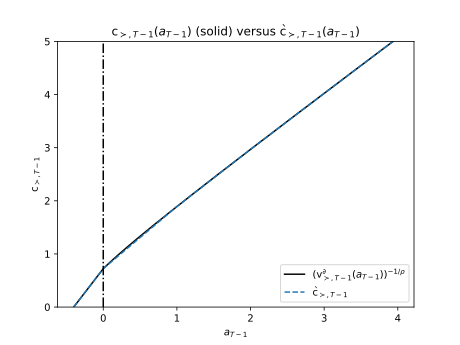
\includegraphics[width=6in]{./Figures/GothVInvVSGothC}}
  \caption{True $\vInv^{a}_{(\prdLsT)_\cntn}(\aNrm)$ vs its approximation $\Aprx{\vInv}^{a}_{(\prdLsT)_\cntn}(\aNrm)$}
  \label{fig:GothVInvVSGothC}
\end{figure}
% \caption{True $\cFunc_{(\prdLsT)_\cntn}(\aNrm)$ vs its approximation $\Aprx{\cFunc}_{(\prdLsT)_\cntn}(\aNrm)$}

Figure \ref{fig:GothVInvVSGothC} shows the result. The solid line calculates the exact numerical value of the consumed function $\cFunc_{(\prdLsT)_\cntn}(\aNrm)$ while the dashed line is the linear interpolating approximation $\Aprx{\cFunc}_{(\prdLsT)_\cntn}(\aNrm).$ This figure illustrates the value of the transformation: The true function is close to linear, and so the linear approximation is almost indistinguishable from the true function except at the very lowest values of $\aNrm$.

Figure~\ref{fig:GothVVSGothCInv} similarly shows that when we generate $\Aprx{\Aprx{\vFunc}}_{(\prdLsT)_\cntn}^{a}(a)$ using our augmented $[\Aprx{\cFunc}_{(\prdLsT)_\cntn}(a)]^{-\CRRA}$ (dashed line) we obtain a \textit{much} closer approximation to the true marginal value function $\vFunc^{a}_{(\prdLsT)_\cntn}(a)$ (solid line) than we obtained in the previous exercise which did not do the transformation (Figure~\ref{fig:PlotOPRawVSFOC}).\footnote{The vertical axis label uses $\mathfrak{v}^{\prime}$ as an alternative notation for what in these notes we designate as $\vFunc^{a}_{\EndPrdLsT}$).  This will be fixed.}
\Fix{\marginpar{\tiny fix the problem articulated in the footnote}}{}

\hypertarget{GothVVSGothCInv}{}
\begin{figure}
  \centerline{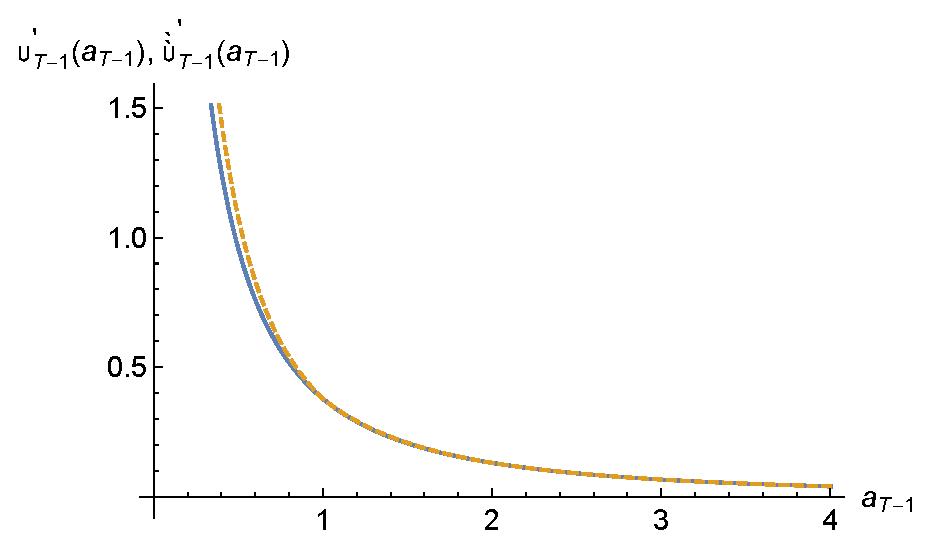
\includegraphics[width=6in]{./Figures/GothVVSGothCInv}}
  \caption{True $\vFunc^{a}_{(\prdLsT)_\cntn}(\aNrm)$ vs. $\Aprx{\Aprx{\vFunc}}_{(\prdLsT)_\cntn}^{a}(\aNrm)$ Constructed Using $\Aprx{\cFunc}_{(\prdLsT)_\cntn}(\aNrm)$}
  \label{fig:GothVVSGothCInv}
\end{figure}

\hypertarget{the-method-of-endogenous-gridpoints}{}
\subsection{The Method of Endogenous Gridpoints (`EGM')}\label{subsec:egm}

The solution procedure we articulated above for finding $\cFunc_{\prdLsT}(m)$ still requires us, for each point in $\vctr{m}\code{_{\prdLsT}}$, to use a numerical rootfinding algorithm to search for the value of $\cNrm$ that solves $\uFunc^{c}(\cNrm) = \vFunc^{a}_{(\prdLsT)_\cntn}(m-\cNrm)$.  Though sections \ref{subsec:transformation} and \ref{subsec:LiqConstrSelfImposed} developed a highly efficient and accurate procedure to calculate $\Aprx{\vFunc}^{a}_{(\prdLsT)_\cntn}$, those approximations do nothing to eliminate the need for using a rootfinding operation for calculating, for an arbitrary $m$, the optimal $c$.  And rootfinding is a notoriously computation-intensive (that is, slow!) operation.

Fortunately, it turns out that there is a way to completely skip this slow rootfinding step.  The method can be understood by noting that we have already calculated, for a set of arbitrary values of $\vctr{a}=\vctr{a}\code{_{\prdLsT}}$, the corresponding $\vctr{c}$ values for which this $\vctr{a}$ is optimal.


But with mutually consistent values of $\vctr{c}\code{_{\prdLsT}}$ and $\vctr{a}\code{_{\prdLsT}}$ (consistent, in the sense that they are the unique optimal values that correspond to the solution to the problem), we can obtain the $\vctr{m}\code{_{\prdLsT}}$ vector that corresponds to both of them from
\begin{equation}\begin{gathered}\begin{aligned}
      \vctr{m}\code{_{\prdLsT}}  & = {\vctr{\cNrm}\code{_{\prdLsT}}+\vctr{a}\code{_{\prdLsT}}}.
    \end{aligned}\end{gathered}\end{equation}

\ifthenelse{\boolean{ToFix}}{\marginpar{\tiny Rename gothic class, maybe to: EndPrd.  Also, harmonize the notation in the notebook in the paper - for example, everwhere in the text we use cNrm for normalized consumption, but for some reason it is capital C in the gothic function.}}{}

These $m$ gridpoints are ``endogenous'' in contrast to the usual solution method of specifying some \textit{ex-ante} (exogenous) grid of values of $\vctr{m}$ and then using a rootfinding routine to locate the corresponding optimal consumption vector $\vctr{c}$.


This routine is performed in the ``Endogenous Gridpoints'' section of the notebook. First, the \texttt{gothic.C\_Tminus1} function is called for each of the pre-specfied values of end-of-period assets stored in \code{aVec}. These values of consumption and assets are used to produce the list of endogenous gridpoints, stored in the object \texttt{mVec\_egm}. With the $\vctr{\cFunc}$ values in hand, the notebook can generate a set of $\vctr{m}\code{_{\prdLsT}}$ and ${\vctr{\cNrm}\code{_{\prdLsT}}}$ pairs that can be interpolated between in order to yield $\Aprx{\cFunc}_{\MidPrdLsT}(\mNrm)$ at virtually zero computational cost!\footnote{This is the essential point of \cite{carrollEGM}.} %This is done in the final line of code in this block, and the following code block produces the graph of the interpolated consumption function using this procedure.

\hypertarget{PlotComparecTm1AD}{}
One might worry about whether the $\{{m},c\}$ points obtained in this way will provide a good representation of the consumption function as a whole, but in practice there are good reasons why they work well (basically, this procedure generates a set of gridpoints that is naturally dense right around the parts of the function with the greatest nonlinearity).
\begin{figure}
  \centerline{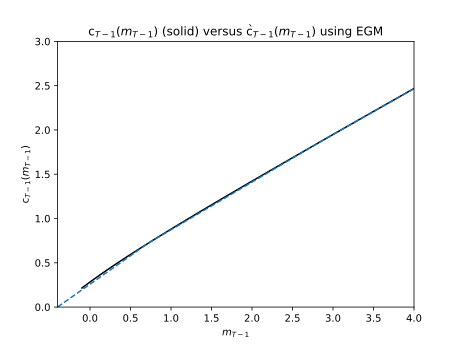
\includegraphics[width=6in]{./Figures/PlotComparecTm1AD}}
  \caption{$\cFunc_{\prdLsT}(m)$ (solid) versus $\Aprx{\cFunc}_{\prdLsT}(m)$ (dashed)}
  \label{fig:ComparecTm1AD}
\end{figure}
Figure~\ref{fig:ComparecTm1AD} plots the actual consumption function $\cFunc_{\prdLsT}$ and the approximated consumption function $\Aprx{\cFunc}_{\prdLsT}$ derived by the method of endogenous grid points. Compared to the approximate consumption functions illustrated in Figure~\ref{fig:PlotcTm1ABC}, $\Aprx{\cFunc}_{\prdLsT}$ is quite close to the actual consumption function.



\hypertarget{improving-the-a-grid}{}
\subsection{Improving the $\aNrm$ Grid}\label{subsec:improving-the-a-grid}

Thus far, we have arbitrarily used $\aNrm$ gridpoints of $\{0.,1.,2.,3.,4.\}$ (augmented in the last subsection by $\NatBoroCnstra_{\prdLsT}$).  But it has been obvious from the figures that the approximated $\Aprx{\cFunc}_{(\prdLsT)_\cntn}$ function tends to be farthest from its true value at low values of $a$.  Combining this with our insight that $\NatBoroCnstra_{\prdLsT}$ is a lower bound, we are now in position to define a more deliberate method for constructing gridpoints for $\aNrm$ -- a method that yields values that are more densely spaced at low values of $a$ where the function is more nonlinear.

A pragmatic choice that works well is to find the values such that (1) the last value \textit{exceeds the lower bound} by the same amount $\bar\aNrm$ as our original maximum gridpoint (in our case, 4.); (2) we have the same number of gridpoints as before; and (3) the \textit{multi-exponential growth rate} (that is, $e^{e^{e^{...}}}$ for some number of exponentiations $n$ -- our default is 3) from each point to the next point is constant (instead of, as previously, imposing constancy of the absolute gap between points).

\hypertarget{GothVInvVSGothCEEE}{}
\begin{figure}
  \centerline{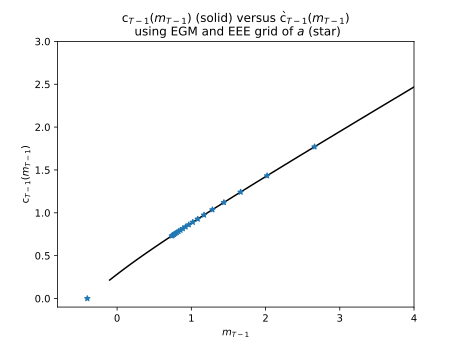
\includegraphics[width=6in]{./Figures/GothVInvVSGothCEEE}}
  \caption{$\cFunc_{(\prdLsT)_\cntn}(\aNrm)$ versus
    $\Aprx{\cFunc}_{(\prdLsT)_\cntn}(\aNrm)$, Multi-Exponential \code{aVec}}
  \label{fig:GothVInvVSGothCEE}
\end{figure}


\hypertarget{GothVVSGothCInvEEE}{}
\begin{figure}
  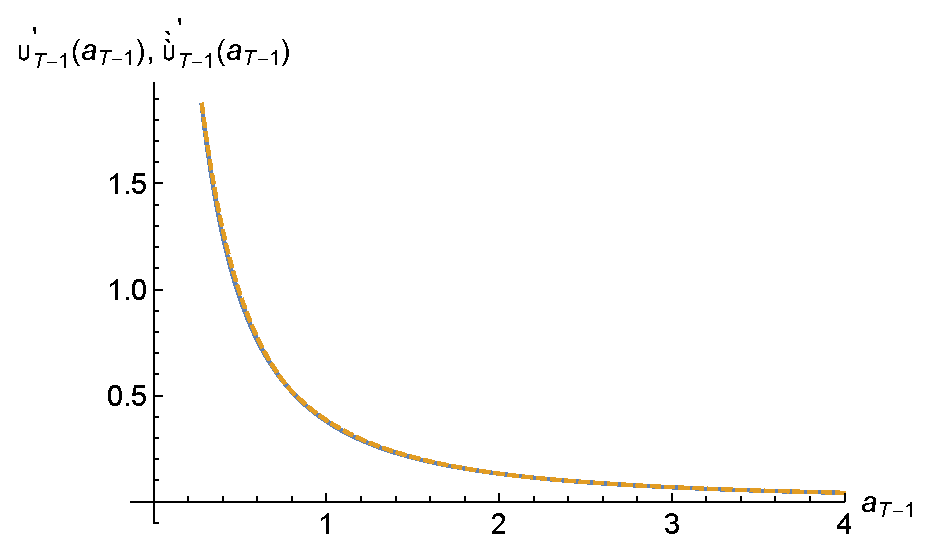
\includegraphics[width=6in]{./Figures/GothVVSGothCInvEEE}
  \caption{$\vFunc^{a}_{(\prdLsT)_\cntn}(\aNrm)$ vs.
    $\Aprx{\Aprx{\vFunc}}_{(\prdLsT)_\cntn}^{a}(\aNrm)$, Multi-Exponential \code{aVec}}
  \label{fig:GothVVSGothCInvEE}
\end{figure}

Section ``Improve the $\mathbb{A}_{grid}$'' begins by defining a function which takes as arguments the specifications of an initial grid of assets and returns the new grid incorporating the multi-exponential approach outlined above.


Notice that the graphs depicted in Figures~\ref{fig:GothVInvVSGothCEE} and \ref{fig:GothVVSGothCInvEE} are notably closer to their respective truths than the corresponding figures that used the original grid.

\subsection{Program Structure}

In section ``Solve for $c_t(\mNrm)$ in Multiple Periods,'' the natural and artificial borrowing constraints are combined with the endogenous gridpoints method to approximate the optimal consumption function for a specific period. Then, this function is used to compute the approximated consumption in the previous period, and this process is repeated for some specified number of periods.

The essential structure of the program is a loop that iteratively solves for consumption functions by working backward from an assumed final period, using the dictionary \texttt{cFunc\_life} to store the interpolated consumption functions up to the beginning period. Consumption in a given period is utilized to determine the endogenous gridpoints for the preceding period. This is the sense in which the computation of optimal consumption is done recursively.

For a realistic life cycle problem, it would also be necessary at a
minimum to calibrate a nonconstant path of expected income growth over the
lifetime that matches the empirical profile; allowing for such
a calibration is the reason we have included the $\{\PermGroFac\}_{\prd}^{T}$
vector in our computational specification of the problem.

\hypertarget{results}{}
\subsection{Results}

The code creates the relevant $\Aprx{\cFunc}_{\prd}(\mNrm)$ functions for any period in the horizon, at the given values of $\mNrm$.  Figure \ref{fig:PlotCFuncsConverge} shows $\Aprx{\cFunc}_{T-n}(m)$ for $n=\{20,15,10,5,1\}$.  At least one feature of this figure is encouraging: the consumption functions converge as the horizon extends, something that \cite{BufferStockTheory} shows must be true under certain parametric conditions that are satisfied by the baseline parameter values being used here.

\hypertarget{PlotCFuncsConverge}{}
\begin{figure}
  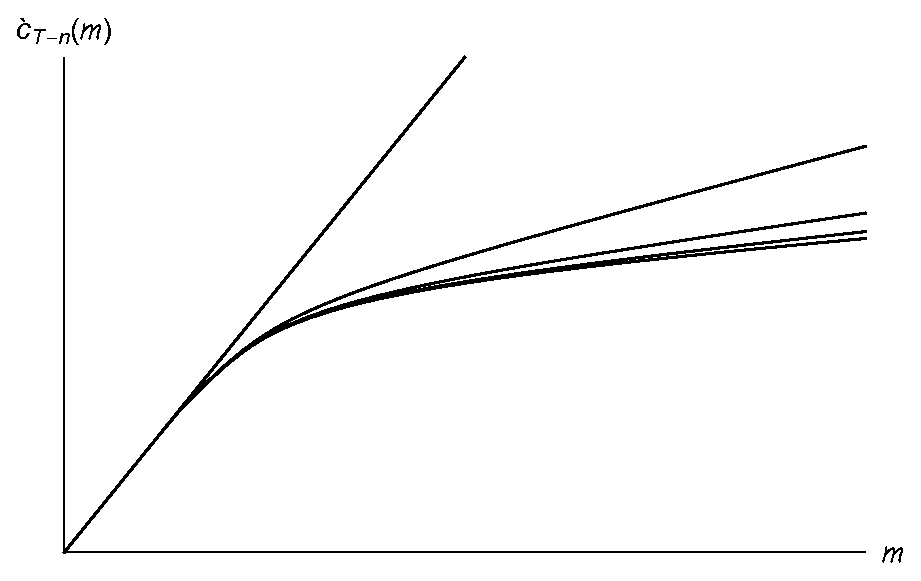
\includegraphics[width=6in]{./Figures/PlotCFuncsConverge}
  \caption{Converging $\Aprx{\cFunc}_{T-n}(\mNrm)$ Functions as $n$ Increases}
  \label{fig:PlotCFuncsConverge}
\end{figure}


\end{document}
